\\documentclass[12pt,a4paper]{article}
\\usepackage[utf8]{inputenc}
\\usepackage{graphicx}
\\usepackage{amsmath}
\\usepackage{caption}
\\usepackage{subcaption}
\\usepackage{geometry}
\\usepackage{booktabs}
\\usepackage{float}
\\geometry{a4paper, margin=1in}

\\title{Experiment 9: Clustering Human Activity Recognition Data using K-Means, DBSCAN, and Hierarchical Clustering}
\\author{Monesh M (Roll No: 3122235001084)}
\\date{\\today}

\\begin{document}

\\maketitle

\\begin{flushright}
  \\textbf{Name:} Monesh M \\\\
  \\textbf{Roll No:} 3122235001084
\\end{flushright}

\\section{Objective}
To implement and analyze the performance of clustering algorithms (K-Means, DBSCAN, and Hierarchical Agglomerative Clustering) on the Human Activity Recognition (HAR) dataset.

\\section{Dataset}
The dataset consists of 10,299 samples, each containing 561 features recorded from smartphone sensors (accelerometer and gyroscope). There are 6 actual activity classes: Walking, Walking Upstairs, Walking Downstairs, Sitting, Standing, and Laying.

\\section{Methodology}
\\begin{itemize}
    \\item \\textbf{Preprocessing:} Features were standardized to zero mean and unit variance.
    \\item \\textbf{Dimensionality Reduction:} PCA was used to project the 561D space into 2D for visual analysis.
    \\item \\textbf{K-Means:} The optimal number of clusters was determined using the Elbow method and Silhouette scores.
    \\item \\textbf{DBSCAN:} A density-based approach was implemented to identify core samples and noise.
    \\item \\textbf{Hierarchical Clustering:} Agglomerative clustering with Ward's linkage was used to build a dendrogram.
\\end{itemize}

\\section{Results and Observations}

\\subsection{K-Means Analysis}
The Elbow method (Figure \\ref{fig:kmeans_analysis}) indicated a significant reduction in inertia (WCSS) around $k=6$, which corresponds to the known number of activities.

\\begin{figure}[H]
    \\centering
    \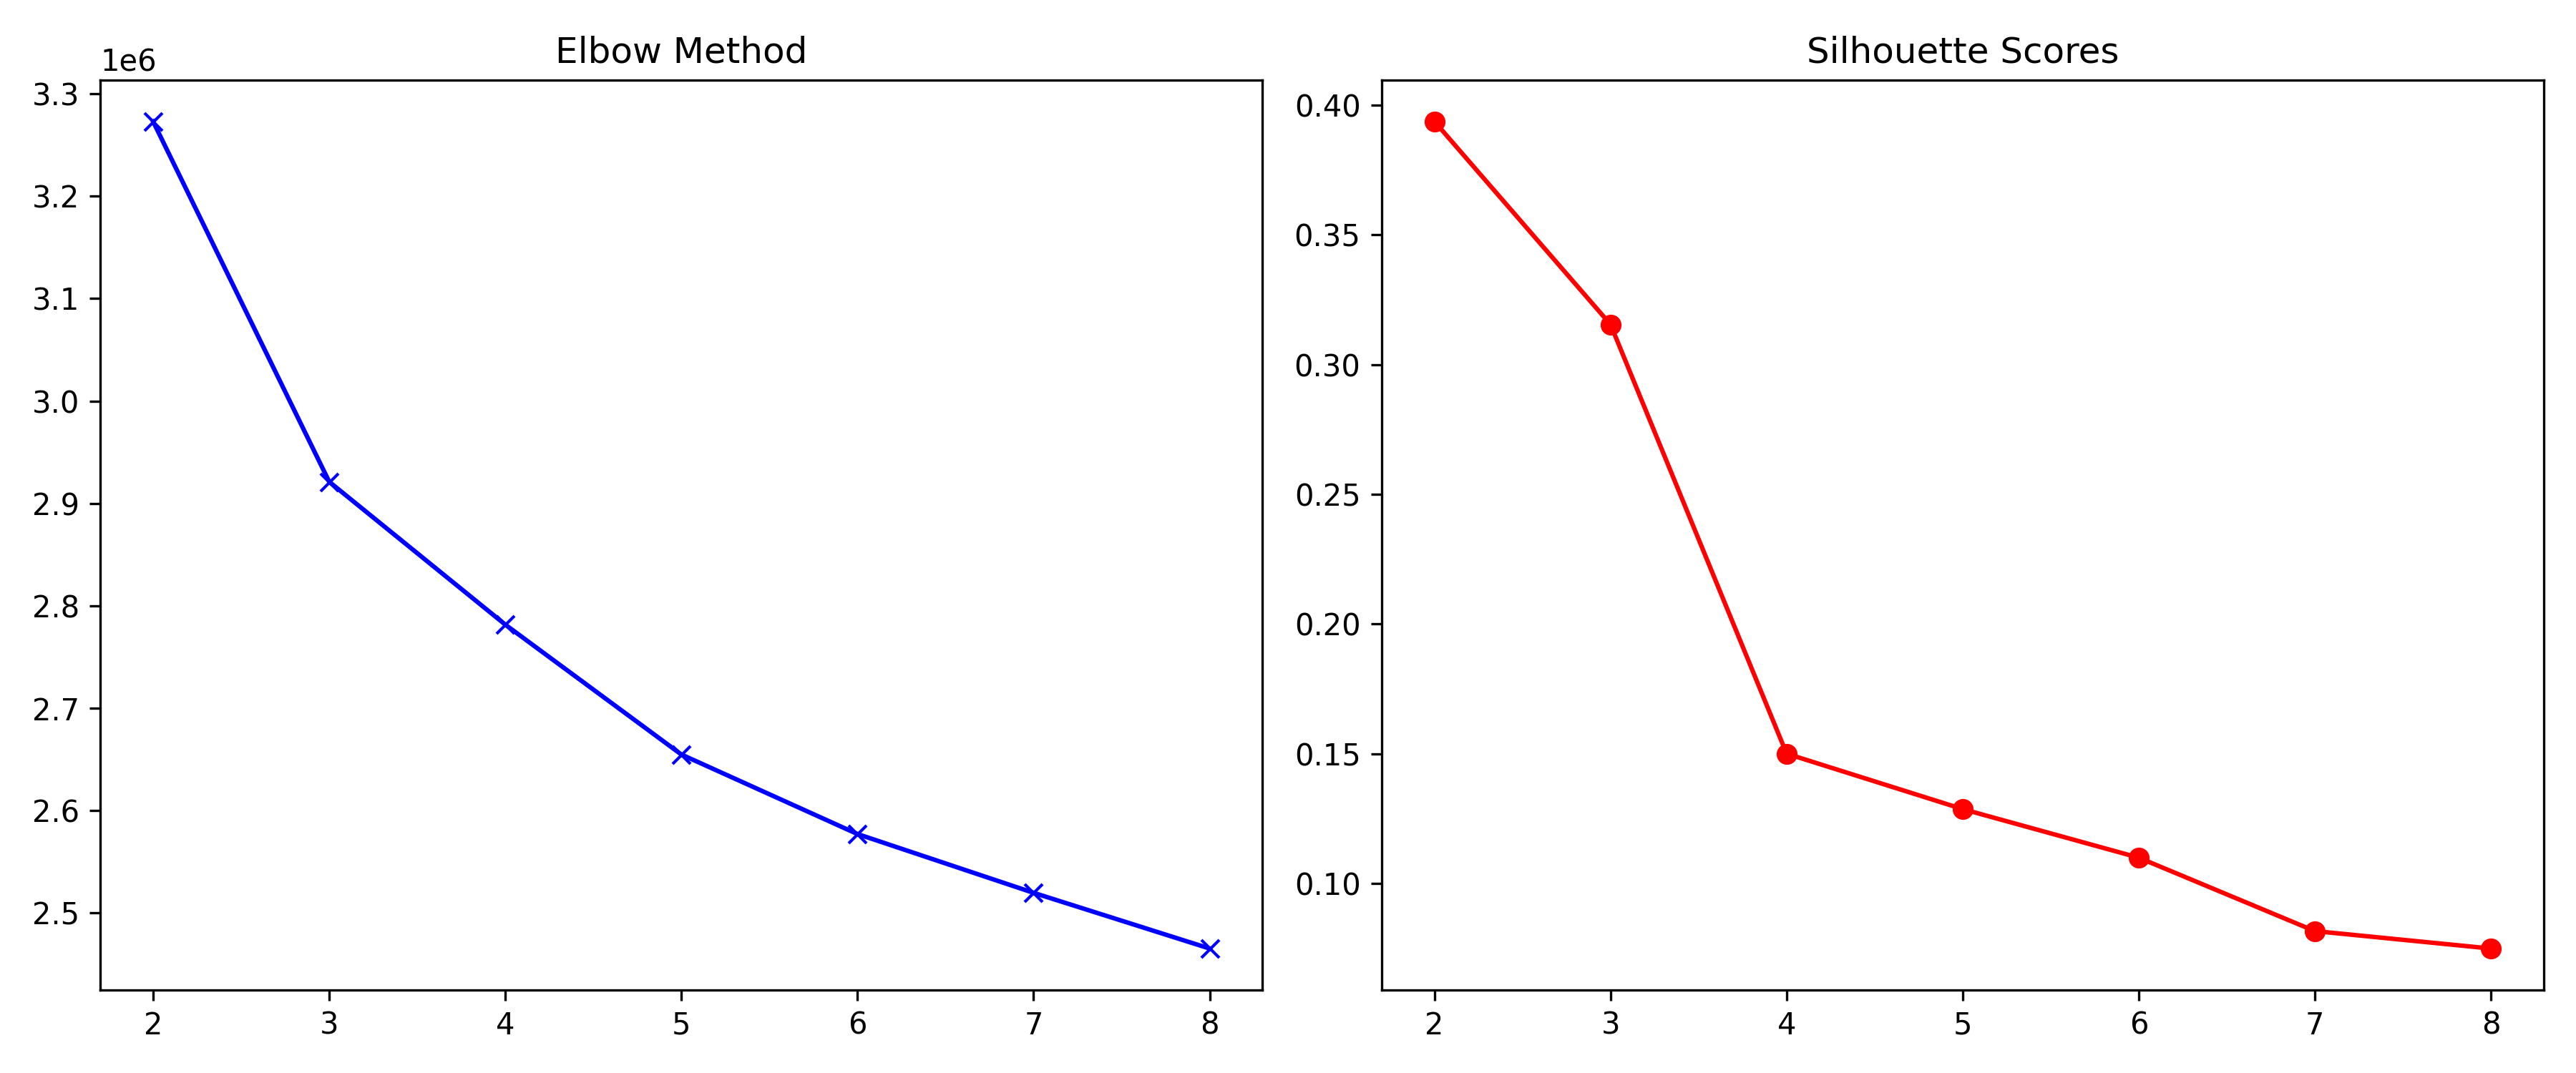
\includegraphics[width=0.8\\textwidth]{images/PNG/kmeans_analysis.png}
    \\caption{Elbow Method and Silhouette Scores for K-Means.}
    \\label{fig:kmeans_analysis}
\\end{figure}

\\subsection{Clustering Performance Metrics}
Table \\ref{tab:comparison} shows the performance comparison of the three algorithms across internal (Silhouette) and external (ARI, NMI) metrics.

\\begin{table}[H]
\\centering
\\caption{Clustering Performance Comparison}
\\label{tab:comparison}
\\begin{tabular}{lcccc}
\\toprule
\\textbf{Algorithm} & \\textbf{Silhouette} & \\textbf{ARI} & \\textbf{NMI} \\\\ 
\\midrule
K-Means ($k=6$) & 0.110 & 0.420 & 0.559 \\\\
DBSCAN & 0.119 & 0.080 & 0.154 \\\\
Hierarchical & 0.117 & 0.460 & 0.601 \\\\
\\bottomrule
\\end{tabular}
\\end{table}

\\section{Visualizations}

\\begin{figure}[H]
    \\centering
    \\begin{subfigure}[b]{0.45\\textwidth}
        \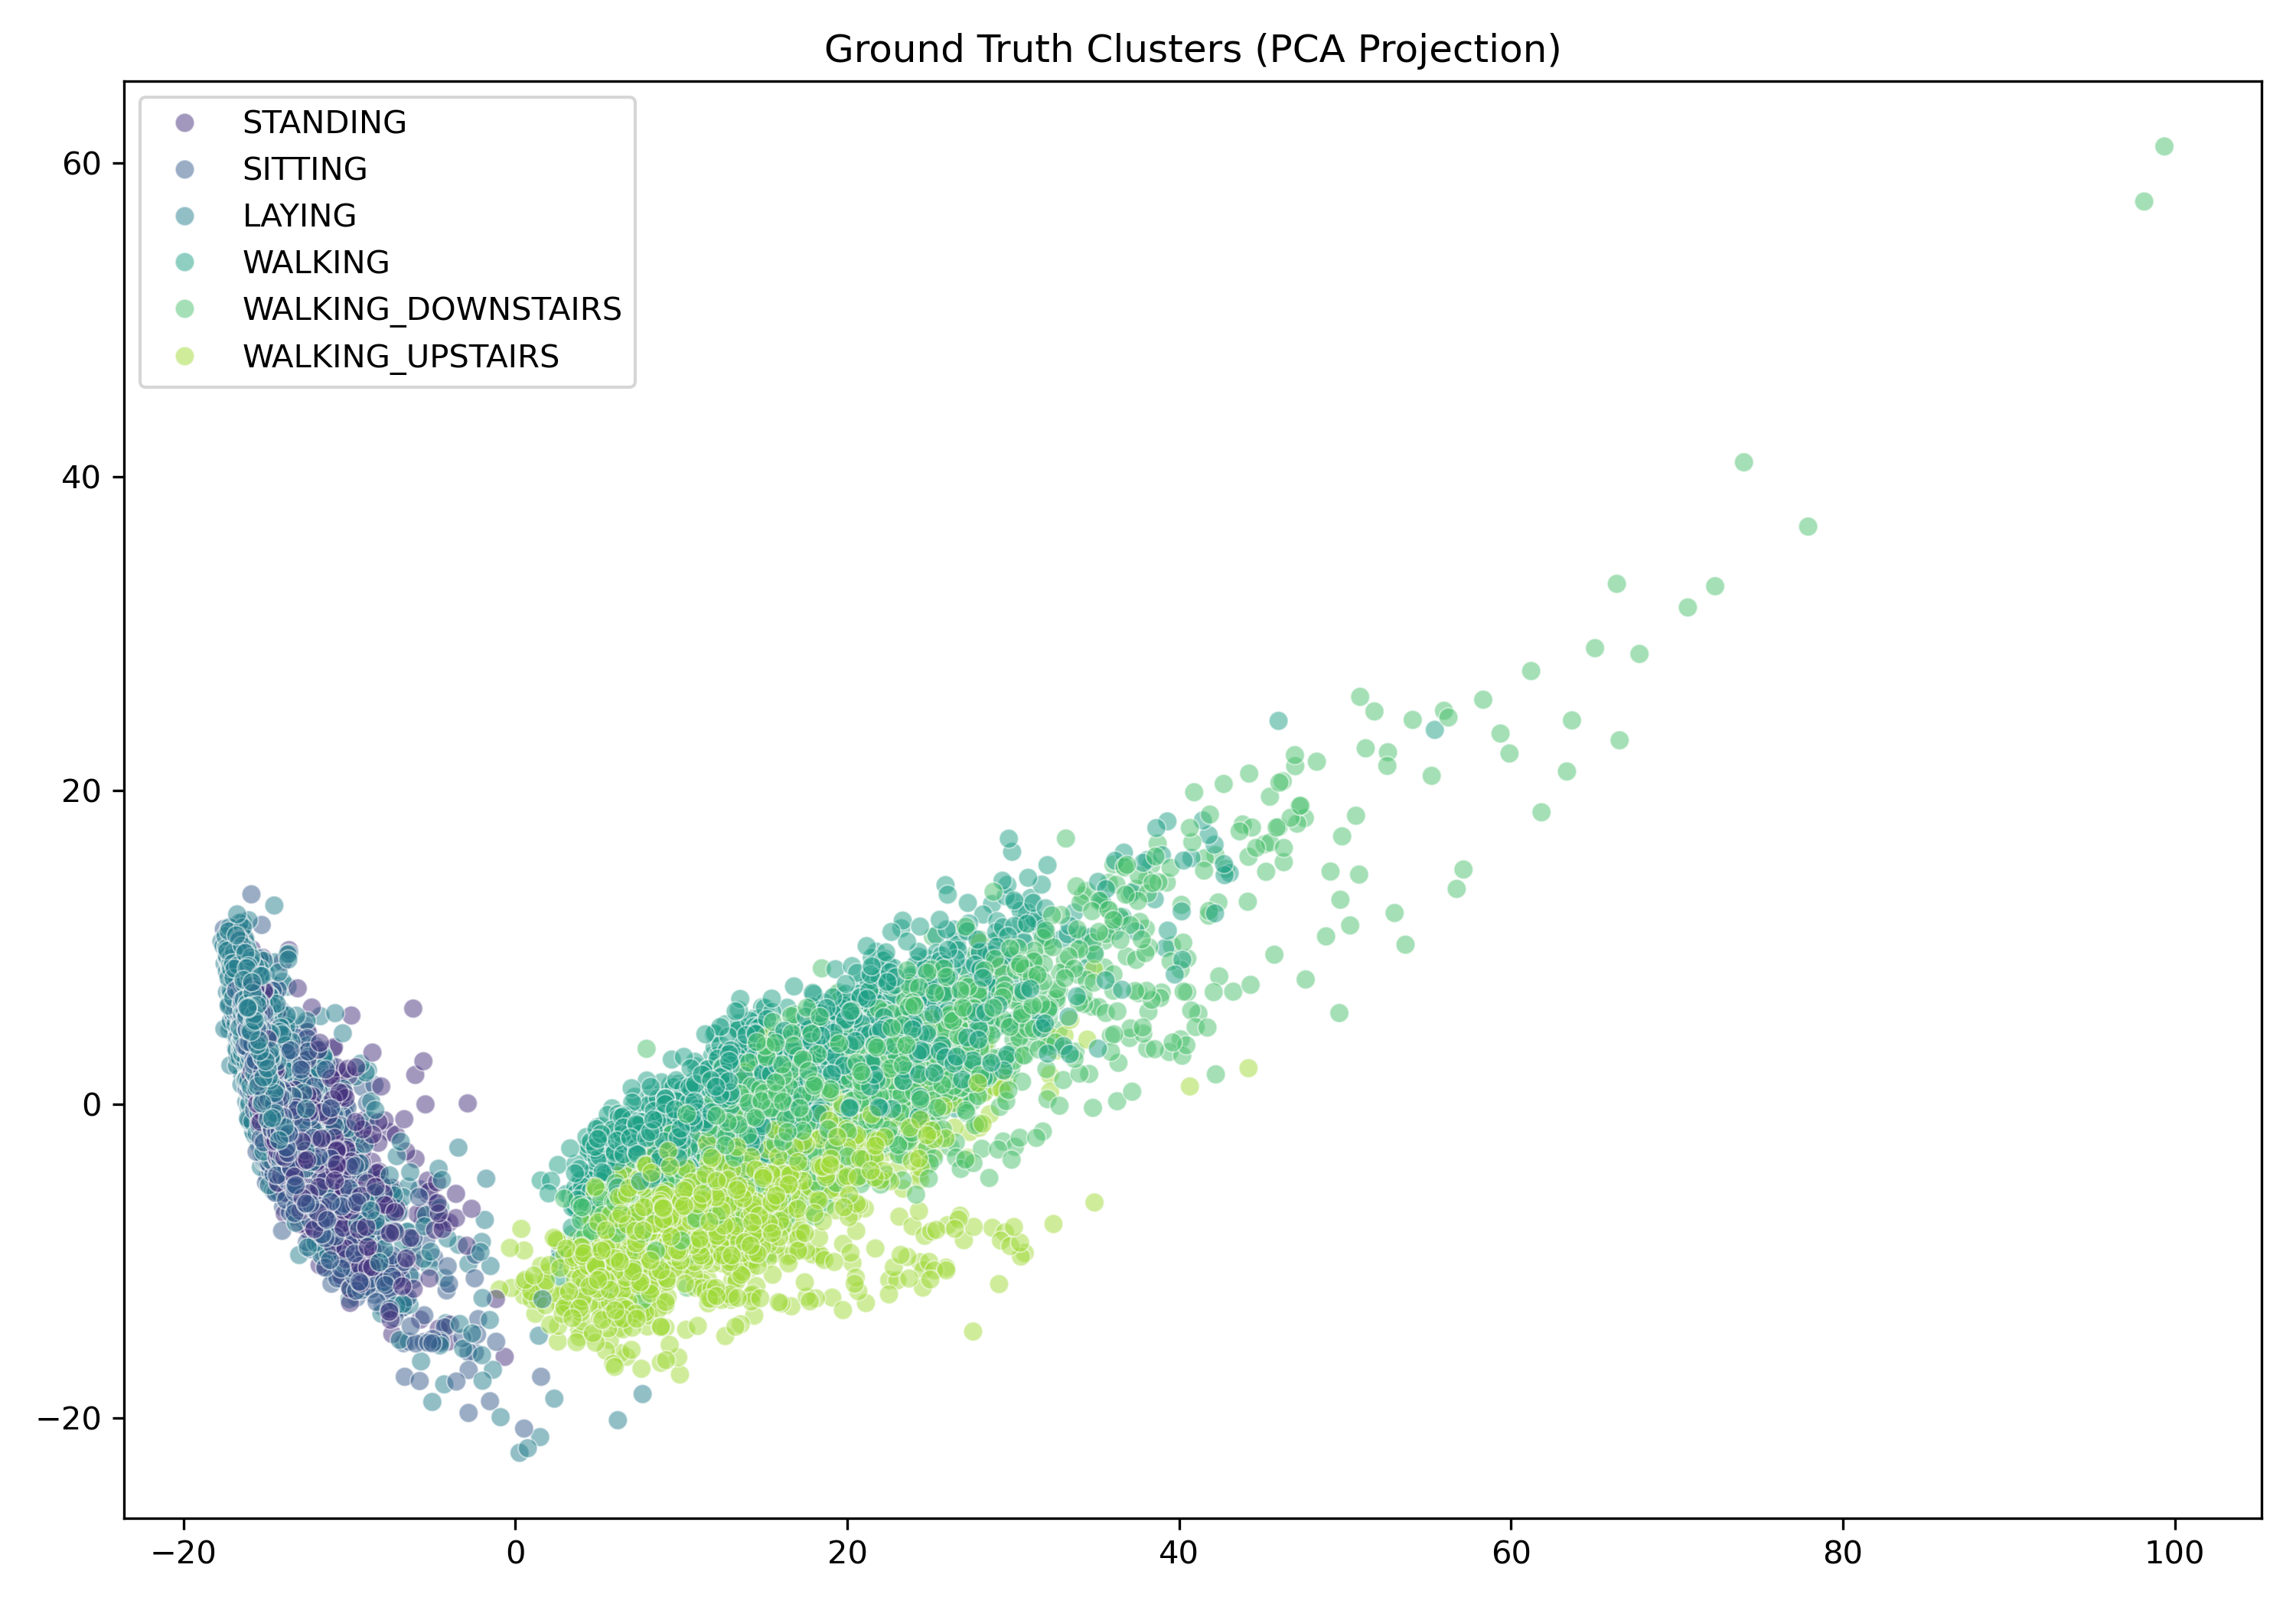
\includegraphics[width=\\textwidth]{images/PNG/pca_ground_truth.png}
        \\caption{Ground Truth (Actual Classes)}
    \\end{subfigure}
    \\hfill
    \\begin{subfigure}[b]{0.45\\textwidth}
        \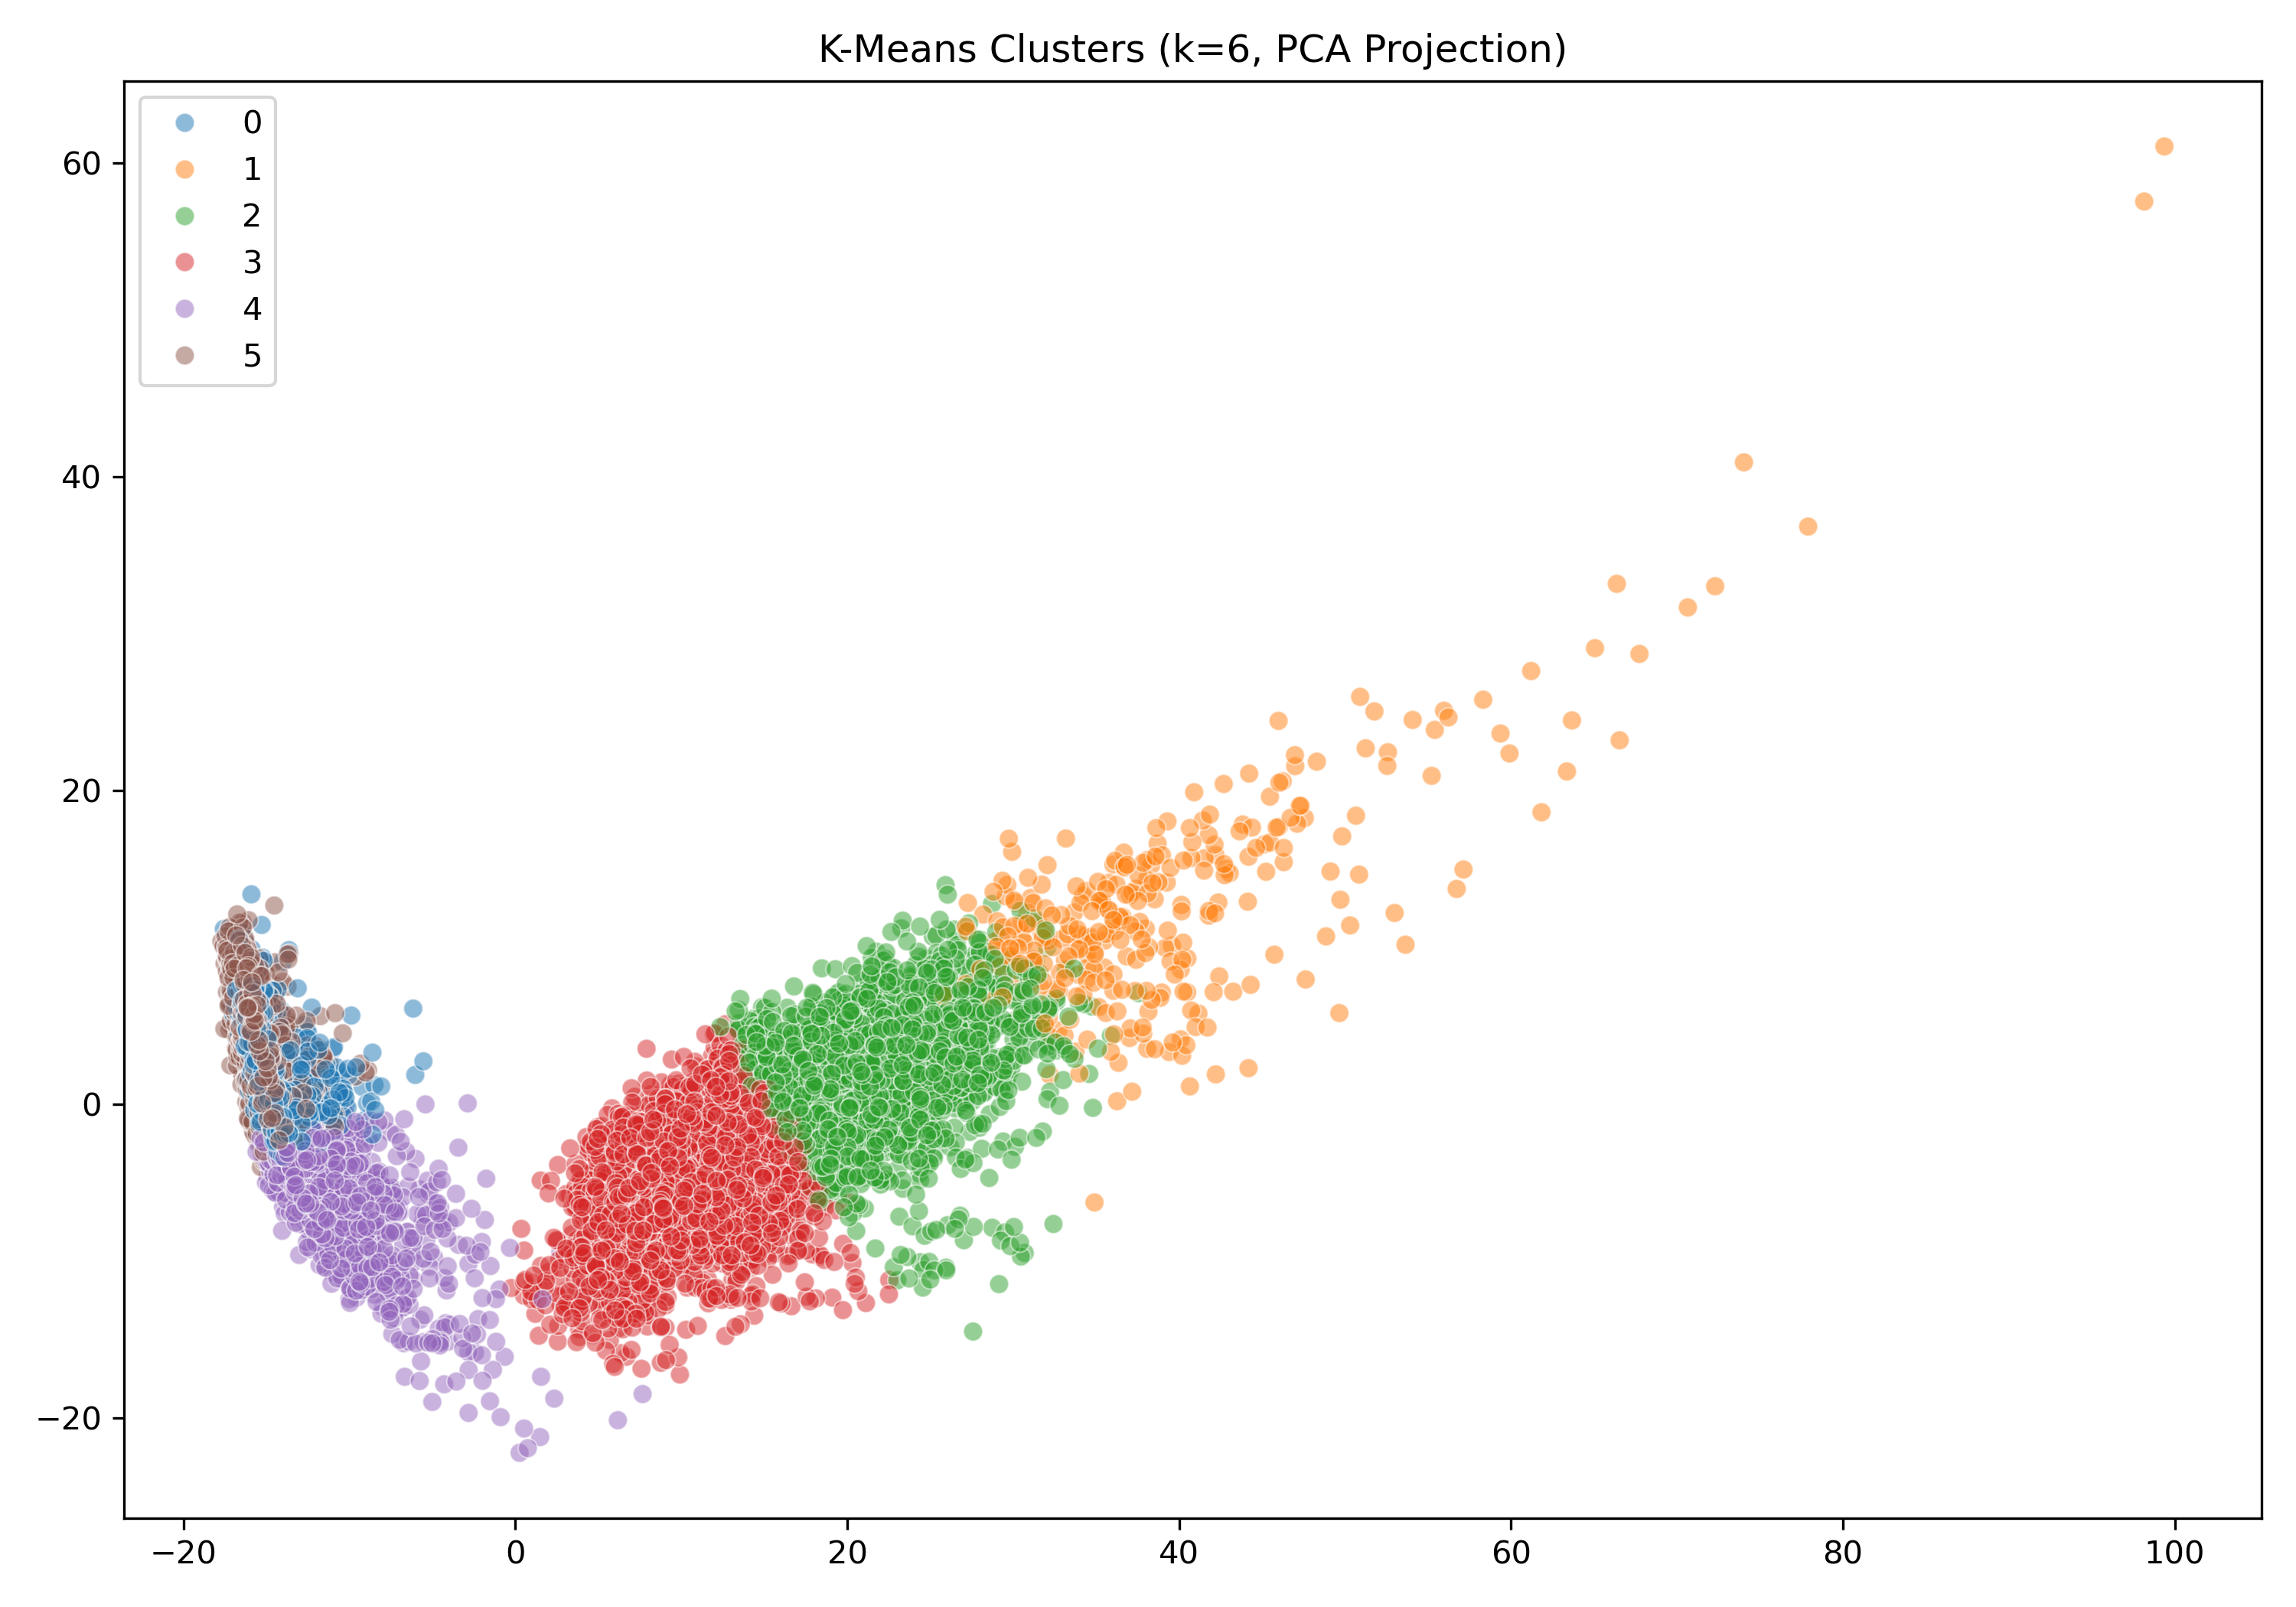
\includegraphics[width=\\textwidth]{images/PNG/kmeans_clusters_pca.png}
        \\caption{K-Means Clusters}
    \\end{subfigure}
    \\caption{PCA Comparison of True Labels vs. K-Means Clusters.}
\\end{figure}

\\begin{figure}[H]
    \\centering
    \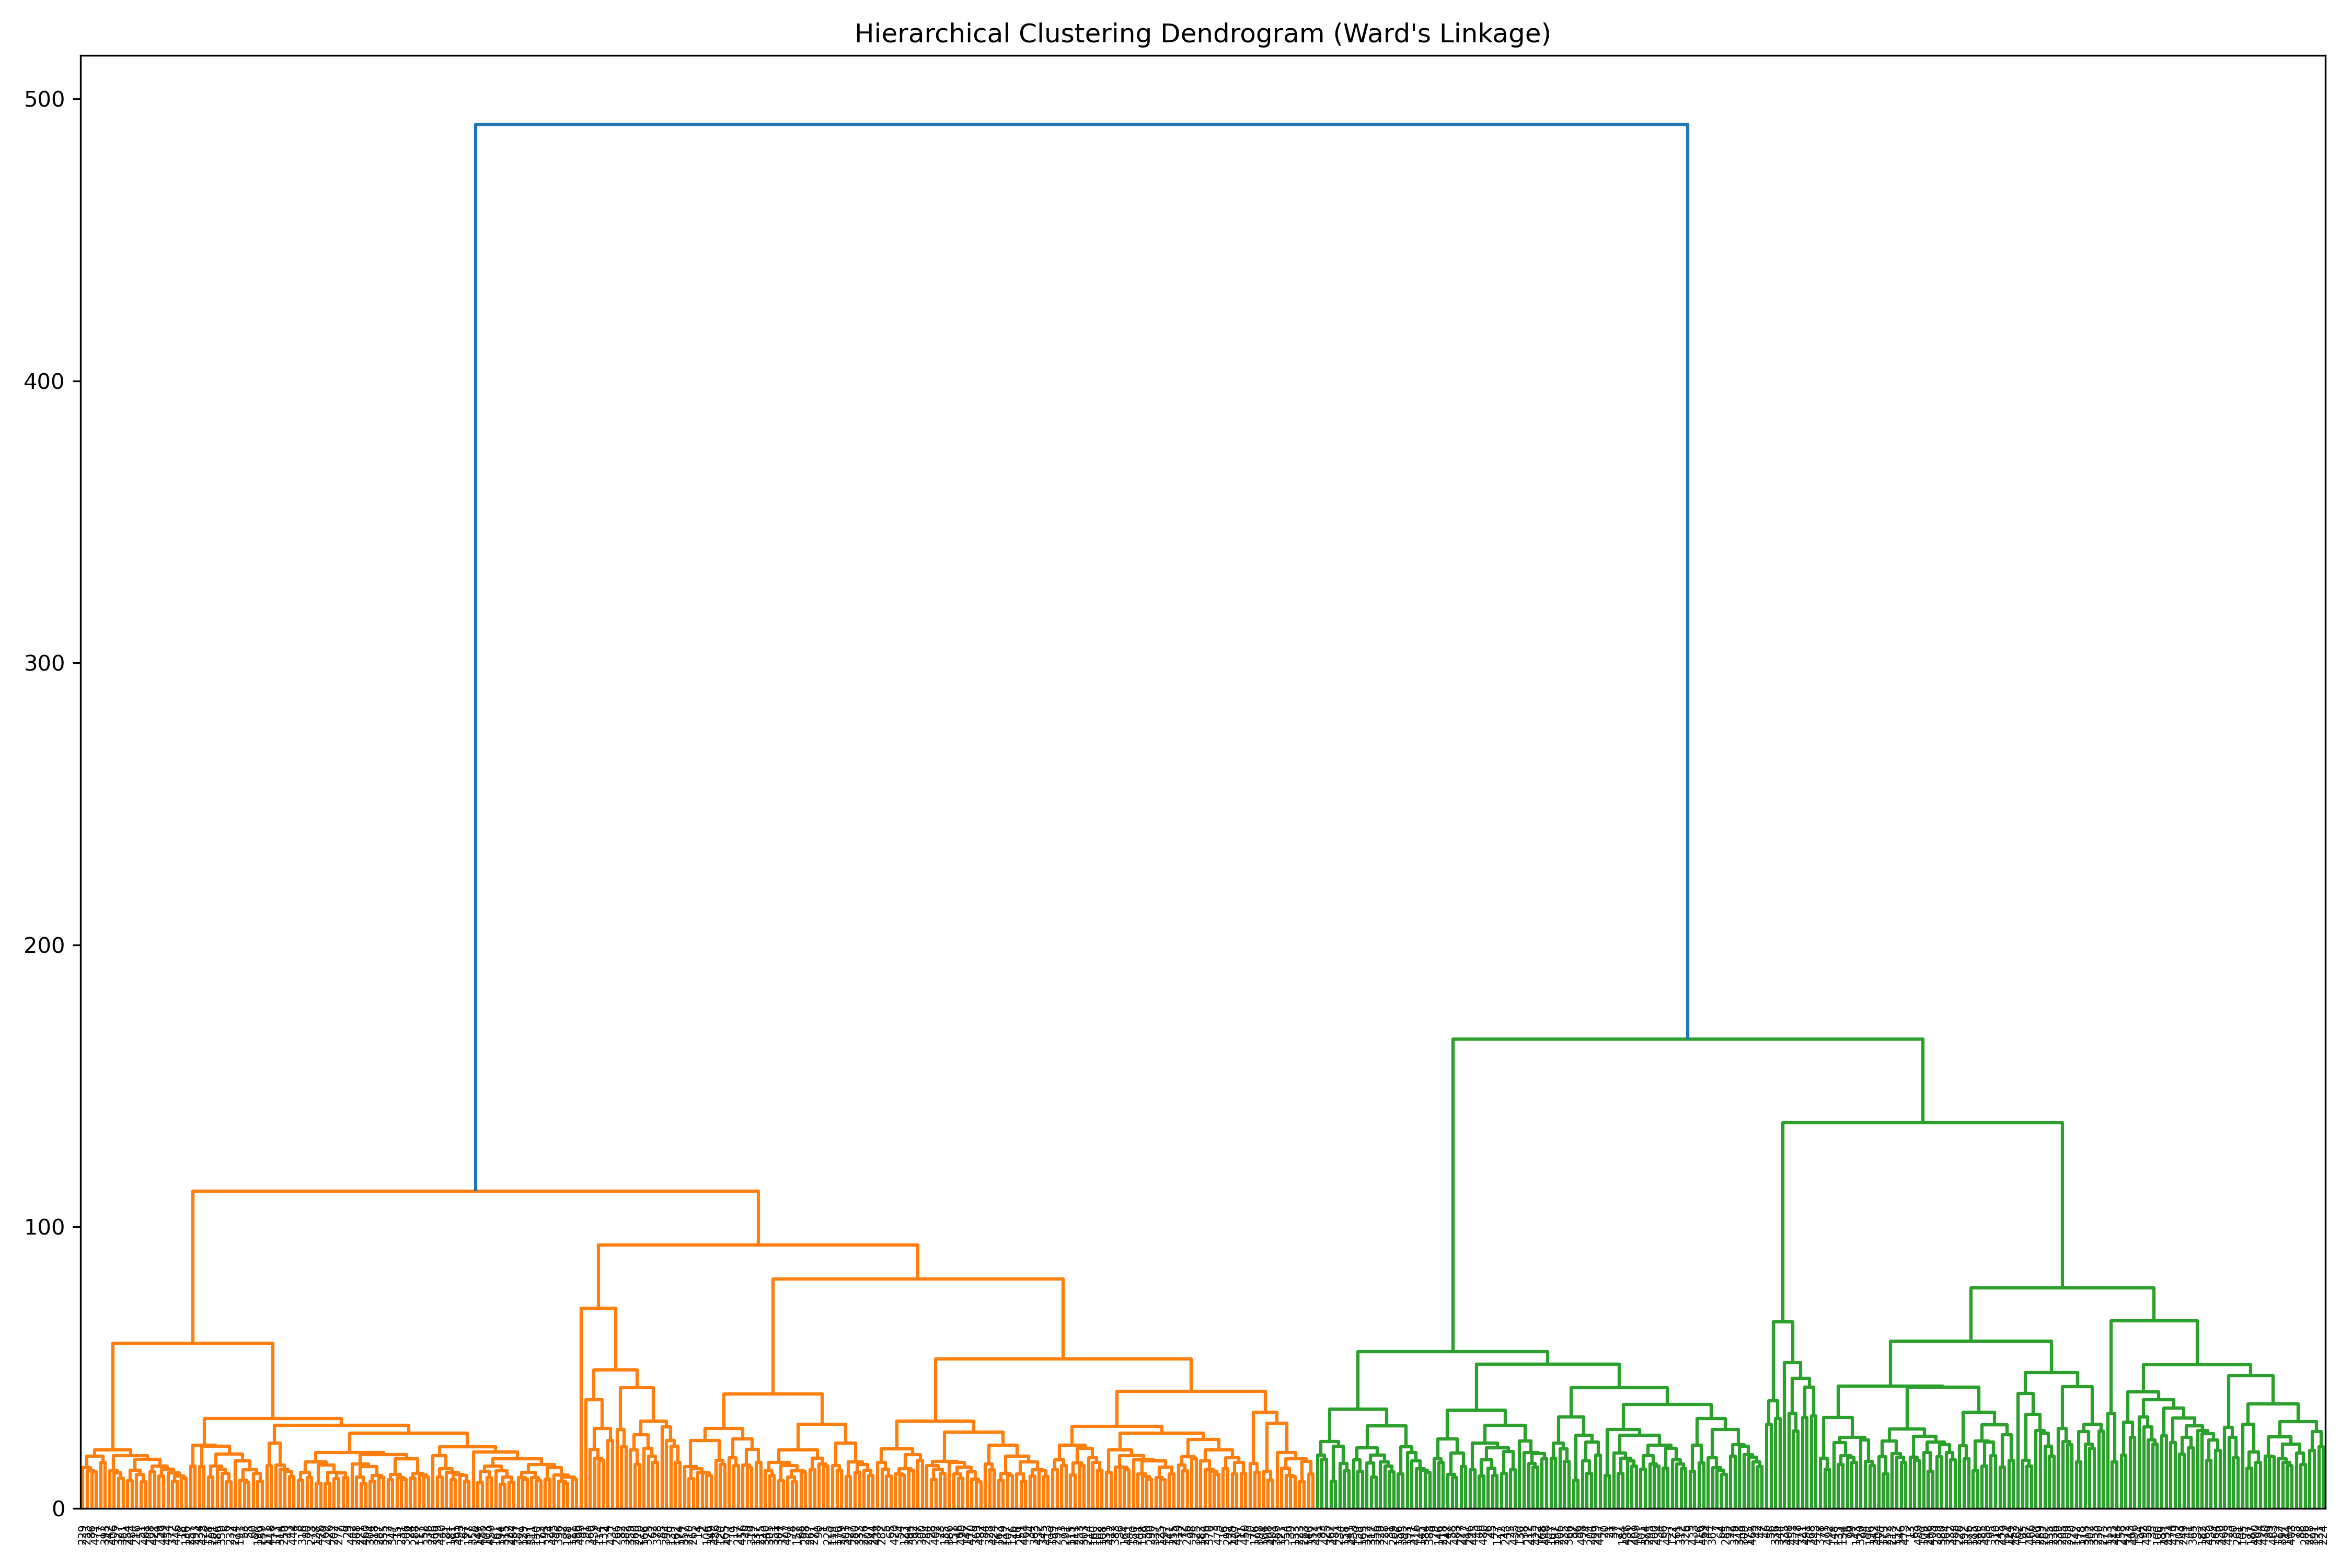
\includegraphics[width=0.8\\textwidth]{images/PNG/hierarchical_dendrogram.png}
    \\caption{Hierarchical Clustering Dendrogram (Ward's Linkage).}
\\end{figure}

\\section{Conclusion}
The analysis reveals that Hierarchical Agglomerative Clustering with Ward's linkage outperformed K-Means and DBSCAN in terms of alignment with ground truth labels (ARI of 0.46 and NMI of 0.60). DBSCAN struggled due to the high-dimensional nature of the dataset.

\\end{document}
